%% v1.1 [2023/09/01]
\documentclass[english]{brccms-hu}
\usepackage{amsmath}
%\usepackage{amsthm}% newtxtext よりも前に読み込む
\usepackage[defaultsups]{newtxtext}
\usepackage[varg]{newtxmath}
\usepackage[dvipdfmx]{graphicx}
%\usepackage[dvips]{graphicx}
\usepackage{xcolor}
\usepackage{url}
\usepackage{cite}
\renewcommand*{\citedash}{$-$\penalty\citepunctpenalty}

\begin{document}
%\Vol{37}
\title{Instructions for Preparing the Manuscript for the Bulletin of\\ Research Center for Computing and Multimedia Studies (RCCMS)\\ Hosei University}
\subtitle{-subtitle-}
\authorlist{%
 \authorentry{First A. Author}{a}
 \authorentry{Second B. Author}{b}
}
\affiliate[a]{Department of ....., University of ...., \Email{e-mail}}
\affiliate[b]{Institute of ....., University of ...., \Email{e-mail}}

%\breakauthorline{4}
%\received{2021}{10}{18}
%\published{2022}{1}{1}

\begin{abstract}
The abstract should be concise and contain an explicit summary of your research that states the problem, the methods used, and the major results and conclusions. It should be single-spaced in 9-point Times New Roman. Be sure to adhere to the word limitation for the abstract (250 words). It is advised to avoid referencing in the abstract (unless it is necessary). Please prepare your manuscript in a \LaTeX{} file following the specific guidelines provided by Research Center for Computing and Multimedia Studies.
\end{abstract}
\begin{keyword}
Research Report, Personal Computer, Word (Please write no more than six keywords.)
\end{keyword}
\maketitle

\section{Introduction}
This document contains the guidelines for preparation of papers for the Bulletin of RCCMS of Hosei University. You must prepare your manuscript carefully according to these instructions. Only papers formatted according to the present guidelines can be accepted. This \LaTeX{} template file is available at the website of RCCMS (https://www.hosei.ac.jp/media/publication/).

This edition was created on 2022/2/1.
\section{Layout and Fonts}
\subsection{Layout}
The prescribed paper size for the electronic file is A4 which is 21.0cm $\times$ 29.7cm. The margins are: top 3cm, bottom 3cm, left and right each 2.5cm. Please make sure that the settings in your word processor and PDF-converter are chosen accordingly. All text must be single spaced. Make use of the maximum stipulated length apart from the following two exceptions: (i) do not begin a new section directly at the bottom of a page, but transfer the heading to the top of the next page; (ii) you may exceed the length of the text area by one line only in order to complete a section of text or a paragraph.
\subsection{Fonts}
The preferred font is “Times-Roman”, the size to be used is 10pt.

The font size of the ‘abstract’ is 9pt. The length of the abstract should not exceed 250 words. Referencing or citations in the abstract is advised to be avoided.
\subsection{Front Matter}
Please keep the headlines before the title line no change. And also, please keep the footer no change. You should start with the title of the paper. The title should be written centered, in 14pt, Times-Roman font. It should be single spaced if the title is more than one line long.

The author's name should include first name, middle initial and surname. It should be written centered, in 12pt Times-Roman font, two lines below the title. Author's affiliation should be written centered, in 9pt, Italic Times-Roman font, one line below the list of authors.

Please write no more than six key words. They should be written left aligned, in 9pt, Times-Roman font, and the line must begin with the words “Keywords:”. Each of the keywords needs to be comma separated. One line space should separate the key words from the summary.
%%%%%%%%%%%%%%%%%%%%%%%%%%%%%%%%%%%%%%%%%%%%%%%%%%%%
\section{Headings}
Use at most three levels of headings which 
correspond to chapters, sections and subsections. The 
main headings should be written Justified, in 10.5pt 
Times-Roman font and preceded by the chapter 
number as “2. Numerical Examples”. There should be 
one lines space before and no line after the main 
headings.
\subsection{Second Headings}
Secondary headings should be written left aligned, 
in 10pt Times-Roman font, with an initial capital like 
“2.1 The Second Level Headings”. There should be 
one line space before and 0.5 line after the secondary 
headings.
\subsubsection{Third Headings}
The third level headings, in 10pt Italic Times-Roman font, are preceded by subsection number like 
“3.1.1 The Third Level Headings”. There should be 0.5 
line space before and 0.5 line after the third headings.
\section{Equations}
A displayed equation is numbered, using Arabic 
numbers in parentheses. It should be centered, leaving 
a 0.5 line space above and below to separate it from 
the surrounding text.

Equations must be typewritten or inserted using 
mathematical editors. Insertion of equations in the 
form of graph, figures and animation must be avoided. 
The following example is a single line equation:

\begin{equation}
    f(x) = \sin x
\end{equation}

The next example is a muli-line equation:

\begin{eqnarray}
    \mathbf{A} \mathbf{x} &=& \mathbf{b}\\
    \int_a^b f(x)dx &=& F(x)
\end{eqnarray}

\begin{table}[htb]
\caption{Example of the Table}
\ecaption{}
\centering
\begin{tabular}{|c|c|}
\hline
caption & font size\\
\hline
table & 10pt\\
\hline
figure & 10pt\\
\hline
\end{tabular}
\end{table}

\begin{figure}[htb]
\centering
% graphic
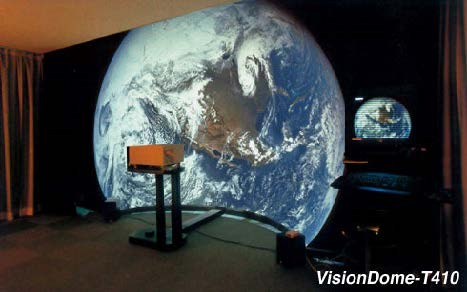
\includegraphics{fig1.jpg}
\caption{Color Figure}
\ecaption{}
\end{figure}

\section{Tables and Figures}
Tables and figures should be originals or sharp 
prints. They should be arranged throughout the text 
and preferably be included on the same page as they 
are first discussed.

All tables should be numbered consecutively and 
captioned. Tables should be centered in the manuscript 
and should have a table caption placed upside (Table 
1). The caption title should be written centered, in 10pt 
Times-Roman font, with an initial capital. 0.5 line 
space should separate the table from the caption, and 
one line space should separate the caption and the 
bottom of the table from the surrounding text.

All figures (diagrams and photographs) should also 
be numbered consecutively and should be placed in the 
text soon after the point where they are referenced. 
Figures should be centered in the manuscript and 
should have a figure caption placed underneath (Fig.1). 
The caption title should be written centered, in 10pt 
Times-Roman font, with an initial capital. 0.5 line 
space should separate the figure from the caption, and 
one line space should separate the upper part of the 
figure and the bottom of the caption from the 
surrounding text.

Animations should be inserted using the same 
guidelines as figures.

For the electronic file to be published on web site, 
it is encouraged to present color pictures. All notations 
and lettering should be no less than 2.5 mm high.
\section{Conclusion}
The Bulletin of RCCMS will be produced from 
those files. So, your manuscript must be free of 
spelling and typing errors. No changes are permitted 
to the paper after submission. Papers not prepared in 
accordance with these instructions will not be 
reviewed and will be returned to the authors.
\section{Footnotes}
Footnotes1 should be placed at the end of the text 
and should be in two columns. The font should be 8pt
“Times-Roman”\footnote{Footnotes should be placed at the end of the text and should 
be in two columns. The font should be 8pt “Times-Roman”}.

\Acknowledgement % Acknowledgement
Acknowledgment (if any) should be followed by 
the conclusions. In accordance with Article 9.2 of the Usage Regulation of Research Center for Computing and Multimedia Studies, Hosei University, “When users publish the results of their research in a paper or other publication, they must clearly state in the paper or other publication that they used the Research Center", please include the following in your acknowledgement. Exaple: This work was used computational resources of the Laboratory provided by the Research Center for Computing and Multimedia Studies, Hosei University (Project ID: LAB-\#\#\#).
\begin{thebibliography}{9}% 文献が10以上のとき99,10未満のとき9など
%Citations should be given according to the examples in the section “REFERENCES” for articles in journals [1] as well as for books [2]. These are based on SIST 02 [3].
%(1) References should be numbered in the order in which they are quoted in the text [1].
%(2) All references should appear together at the end of paper as shown in the example below [1].
%(3) The reference should be written single-spaced, justified, using 9pt Times-Roman in one column.
%(4) More than two referencing (for consecutive sources) should be cited as [1]-[4] instead of [1][2][3][4]. 
%Example are as follows
\bibitem{1} Hughes, T.J.R. Generalization of selective integration 
procedures to anisotropic and nonlinear media. Int. J. 
Numer. Meth. Engrg. 1980, 15, p. 1413-1418.
\bibitem{2} Zienkiewicz, O.C. and Taylor, R.L. The Finite Element 
Methods. 4th ed., McGraw-Hill Co., Ltd, 1991
\bibitem{3}  “Description of References SIST 02-2007”. Japan Science and Technology Agency. \url{https://warp.ndl.go.jp/info:ndljp/pid/12003258/jipsti.jst.go.jp/sist/handbook/sist02_2007/main.htm}, (accessed 2022-05-17). (Japanese).
\end{thebibliography}

\appendix
Appendix should be placed after Acknowledgment 
and References
\end{document}